\documentclass[UTF8]{article}
\usepackage{graphicx}
\usepackage{subfigure}
\usepackage{amsmath}
\usepackage{makecell}
\usepackage[utf8]{inputenc}
\usepackage[space]{ctex} %中文包
\usepackage{listings} %放代码
\usepackage{xcolor} %代码着色宏包
\usepackage{CJK} %显示中文宏包
\usepackage{float}
\usepackage{diagbox}
\usepackage{bm}
\usepackage{ulem} 
\usepackage{amssymb}
\usepackage{soul}
\usepackage{color}
\usepackage{geometry}
\usepackage{fancybox} %花里胡哨的盒子
\usepackage{xhfill} %填充包, 可画分割线 https://www.latexstudio.net/archives/8245
\usepackage{multicol} %多栏包
\usepackage{enumerate} %可以方便地自定义枚举标题
\usepackage{multirow} %表格中多行单元格合并
\usepackage{wasysym} %可以使用wasysym里的一堆奇奇怪怪的符号
\usepackage{hyperref} % url
%%%%%%%%%%%%%%%伪代码%%%%%%%%%%%%%%%
\usepackage{amsmath}
\usepackage{algorithm}
\usepackage{algorithmicx}
\usepackage[noend]{algpseudocode}
%%%%%%%%%%%%%%%画图包%%%%%%%%%%%%%%%
\usepackage{tikz}
\usepackage{pgfplots} % http://pgfplots.sourceforge.net/gallery.html
\usetikzlibrary{pgfplots.patchplots} % 拟合支持
\usetikzlibrary{arrows,shapes,automata,petri,positioning,calc} % 状态图支持
\usetikzlibrary{arrows.meta} % 箭头
\usetikzlibrary{shadows} % 阴影支持
\usepackage{forest} % 画树

\geometry{left = 1.5cm, right = 1.5cm, top=1.5cm, bottom=2cm}

\definecolor{mygreen}{rgb}{0,0.6,0}
\definecolor{mygray}{rgb}{0.5,0.5,0.5}
\definecolor{mymauve}{rgb}{0.58,0,0.82}
\lstset{
	backgroundcolor=\color{white}, 
	%\tiny < \scriptsize < \footnotesize < \small < \normalsize < \large < \Large < \LARGE < \huge < \Huge
	basicstyle = \tiny,       
	breakatwhitespace = false,        
	breaklines = true,                 
	captionpos = b,                    
	commentstyle = \color{mygreen}\bfseries,
	extendedchars = false,
	frame = shadowbox, 
	framerule=0.5pt,
	keepspaces=true,
	keywordstyle=\color{blue}\bfseries, % keyword style
	language = C++,                     % the language of code
	otherkeywords={string}, 
	numbers=left, 
	numbersep=5pt,
	numberstyle=\tiny\color{mygray},
	rulecolor=\color{black},         
	showspaces=false,  
	showstringspaces=false, 
	showtabs=false,    
	stepnumber=1,         
	stringstyle=\color{mymauve},        % string literal style
	tabsize=4,          
	title=\lstname           
}

%\sum\nolimits_{j=1}^{M}   上下标位于求和符号的水平右端,
%\sum\limits_{j=1}^{M}   上下标位于求和符号的上下处,
%\sum_{j=1}^{M}  对上下标位置没有设定,会随公式所处环境自动调整。

%%%%%%%%%%%%%画图包%%%%%%%%%%%%%
\usepackage{tikz}
%%%%%%%%%%%%%好看的矩形%%%%%%%%%%%%%
\tikzset{
  rect1/.style = {
    shape = rectangle,% 指定样式
    minimum height=2cm,% 最小高度
    minimum width=4cm,% 最小宽度
    align = center,% 文字居中
    drop shadow,% 阴影
  }
}
%%%%%%%%%%%%%画图背景包%%%%%%%%%%%%%
\usetikzlibrary{backgrounds}

%%%%%%%%%%%%%在tikz中画一个顶点%%%%%%%%%%%%%
%%%%%%%%%%%%%#1:node名称%%%%%%%%%%%%%
%%%%%%%%%%%%%#2:位置%%%%%%%%%%%%%
%%%%%%%%%%%%%#3:标签%%%%%%%%%%%%%
\newcommand{\newVertex}[3]{\node[circle, draw=black, line width=1pt, scale=0.8] (#1) at #2{#3}}
%%%%%%%%%%%%%在tikz中画一条边%%%%%%%%%%%%%
\newcommand{\newEdge}[2]{\draw [black,very thick](#1)--(#2)}
%%%%%%%%%%%%%在tikz中放一个标签%%%%%%%%%%%%%
%%%%%%%%%%%%%#1:名称%%%%%%%%%%%%%
%%%%%%%%%%%%%#2:位置%%%%%%%%%%%%%
%%%%%%%%%%%%%#3:标签内容%%%%%%%%%%%%%
\newcommand{\newLabel}[3]{\node[line width=1pt] (#1) at #2{#3}}

%%%%%%%%%%%%%强制跳过一行%%%%%%%%%%%%%
\newcommand{\jumpLine} {\hspace*{\fill} \par}
%%%%%%%%%%%%%关键点指令,可用itemise替代%%%%%%%%%%%%%
\newcommand{\keypoint}[2]{$\bullet$\textbf{#1}\quad#2\par}
%%%%%%%%%%%%%<T>平均值表示%%%%%%%%%%%%%
\newcommand{\average}[1]{\left\langle #1\right\rangle }
%%%%%%%%%%%%%表格内嵌套表格%%%%%%%%%%%%%
\newcommand{\tabincell}[2]{\begin{tabular}{@{}#1@{}}#2\end{tabular}}
%%%%%%%%%%%%%大黑点item头%%%%%%%%%%%%%
\newcommand{\itemblt}{\item[$\bullet$]}
%%%%%%%%%%%%%大圈item头%%%%%%%%%%%%%
\newcommand{\itemc}{\item[$\circ$]}
%%%%%%%%%%%%%大星星item头%%%%%%%%%%%%%
\newcommand{\itembs}{\item[$\bigstar$]}
%%%%%%%%%%%%%右▷item头%%%%%%%%%%%%%
\newcommand{\itemrhd}{\item[$\rhd$]}
%%%%%%%%%%%%%定义为%%%%%%%%%%%%%
\newcommand{\defas}{=_{df}}
%%%%%%%%%%%%%偏导%%%%%%%%%%%%%
\newcommand{\partialx}[2]{\frac{\partial #1}{\partial #2}}
%%%%%%%%%%%%%蕴含%%%%%%%%%%%%%
\newcommand{\imp}{\rightarrow}
%%%%%%%%%%%%%上取整%%%%%%%%%%%%%
\newcommand{\ceil}[1]{\lceil#1\rceil}
%%%%%%%%%%%%%下取整%%%%%%%%%%%%%
\newcommand{\floor}[1]{\lfloor#1\rfloor}

%%%%%%%%%%%%%双线分割线%%%%%%%%%%%%%
\newcommand*{\doublerule}{\hrule width \hsize height 1pt \kern 0.5mm \hrule width \hsize height 2pt}
%%%%%%%%%%%%%双线中间可加东西的分割线%%%%%%%%%%%%%
\newcommand\doublerulefill{\leavevmode\leaders\vbox{\hrule width .1pt\kern1pt\hrule}\hfill\kern0pt }
%%%%%%%%%%%%%左大括号%%%%%%%%%%%%%
\newcommand{\leftbig}[1]{\left\{\begin{array}{l}#1\end{array}\right.}
%%%%%%%%%%%%%矩阵%%%%%%%%%%%%%
\newcommand{\mat}[2]{\left[\begin{array}{#1}#2\end{array}\right]}
%%%%%%%%%%%%%可换行圆角文本框%%%%%%%%%%%%%
\newcommand{\ovalboxn}[1]{\ovalbox{\tabincell{l}{#1}}}
%%%%%%%%%%%%%设置section的counter, 使从1开始%%%%%%%%%%%%%
\setcounter{section}{0}

%%%%%%%%%%%%%Colors%%%%%%%%%%%%%
\newcommand{\lightercolor}[3]{% Reference Color, Percentage, New Color Name
    \colorlet{#3}{#1!#2!white}
}
\newcommand{\darkercolor}[3]{% Reference Color, Percentage, New Color Name
    \colorlet{#3}{#1!#2!black}
}
\definecolor{aquamarine}{rgb}{0.5, 1.0, 0.83}
\definecolor{Seashell}{RGB}{255, 245, 238} %背景色浅一点的
\definecolor{Firebrick4}{RGB}{255, 0, 0}%文字颜色红一点的
\lightercolor{gray}{20}{lgray}
\newcommand{\hlg}[1]{
	\begingroup
		\sethlcolor{lgray}%背景色
		\textcolor{black}{\hl{\mbox{#1}}}%textcolor里面对应文字颜色
	\endgroup
}


\title{机器学习概论 实验报告 \\ \Large Lab1: LR}

\begin{document}
\maketitle
\tableofcontents
\newpage
\section{实验简介}
\noindent 本实验为 \hlg{Logistics Regression} 模型实现实验, 我们的目标是根据 Horse-colic 数据集中的部分样本作回归, 以梯度上升法为基础, 并用测试集测试精确度.
\section{理论基础}
\subsection{多元回归方程形式}
\noindent 多元回归方程形式:
$$y=\beta_0+\beta_1x_1+\beta_2x_2+\cdots+\beta_px_p$$
写成矩阵形式为:
$$\bm{Y}=\bm{X}\bm{\beta}$$
\subsection{Logistics Regression 模型}
\noindent Logistics Regression 模型中, 利用了 \hlg{sigmoid} 函数来估计概率
$$P(\bm{Y}=1)=\frac{1}{1+e^{\bm{X}\bm{\beta}}}$$
为了估计出参数 $\bm{\beta}$, 课本采用了 \hlg{最大似然估计}. 以二分类问题为例, 我们有:
$$P(y|x,\beta)=P(y=1|x,\beta)^y[1-P(y=1|x,\beta)]^{1-y}$$
由此可以写出似然函数:
$$\mathcal{L}(\beta)=\prod\limits_{i=1}^nP(y_i|x_i,\beta)=\prod\limits_{i=1}^n\left(\frac{1}{1+e^{-x_i\beta}}\right)^{y_i}\left(1-\frac{1}{1+e^{-x_i\beta}}\right)^{1-y_i}$$
对其取对数即得到对数似然函数:
$$\log\mathcal{L}(\beta)=\sum\limits_{i=1}^n\left[y_i\log\left(\frac{1}{1+e^{-x_i\beta}}\right) + (1-y_i)\log\left(1-\frac{1}{1+e^{-x_i\beta}}\right)\right]$$
我们可以将它的相反数当做损失函数:
$$J(\beta)=-\log\mathcal{L}(\beta)=-\sum\limits_{i=1}^n\left[y_i\log\left(P(y_i)\right) + (1-y_i)\log\left(1-P(y_i)\right)\right]$$
\subsection{优化方法}
\noindent 为了用梯度法优化参数, 应当将损失函数对参数 $\beta$ 求导:
$$\partialx{J(\beta)}{\beta_j}=-\sum\limits_{i=1}^n(y_i-f(x_i,\beta))\cdot x_{ij}=\sum\limits_{i=1}^n\left(\frac{1}{1+e^{-x_i\beta}}-y_i\right)\cdot x_{ij}$$
然后根据梯度下降法的原理:
$$\beta_{t+1}\leftarrow \beta_{t}-\alpha\nabla J(\beta)$$
即可进行迭代优化. 当然也可以使用 SGD 或 Newton法进行优化.
\section{优化算法}
\subsection{Gradient Descent 算法(GD)}
\begin{algorithm}[H]
	\caption{GD}
	\begin{algorithmic}[1] %每行显示行号
		\Require 训练的 epochs $T$; 初始化 $\beta=(w,b)$, 学习率 $\alpha$
		\For{每个 epoch}
			\State $d\beta = 0$
			\For{每个训练样本 $x_i$}
				\State $d\beta = d\beta + \sum\limits_{i=1}^n\left(\frac{1}{1+e^{-x_i\beta}}-y_i\right)\cdot x_{ij}$
			\EndFor
			\State $\beta = \beta - \alpha * d\beta$
		\EndFor
	\end{algorithmic}
\end{algorithm}
\subsection{Stochastic Gradient Descent 算法(SGD)}
\begin{algorithm}[H]
	\caption{SGD}
	\begin{algorithmic}[1] %每行显示行号
		\Require 训练的 epochs $T$; 初始化 $\beta=(w,b)$, 学习率 $\alpha$
		\For{每个 epoch}
			\State $d\beta = 0$
			\State 随机选定样本序号 $i$
			\State $d\beta = d\beta + -\sum\limits_{i=1}^n(y_i-f(x_i,\beta))\cdot x_{ij}=\sum\limits_{i=1}^n\left(\frac{1}{1+e^{-x_i\beta}}-y_i\right)\cdot x_{ij}$
			\State $\beta = \beta - \alpha * d\beta$
		\EndFor
	\end{algorithmic}
\end{algorithm}
\subsection{Newton法}
\begin{algorithm}[H]
	\caption{Newton}
	\begin{algorithmic}[1] %每行显示行号
		\Require 训练的 epochs $T$; 初始化 $\beta=(w,b)$, 学习率 $\alpha$
		\For{每个 epoch}
			\State $d\beta = 0$
			\State $dd\beta=0$
			\For{每个训练样本 $x_i$}
				\State $d\beta = d\beta + \sum\limits_{i=1}^n\left(\frac{1}{1+e^{-x_i\beta}}-y_i\right)\cdot x_{ij}$
				\State $dd\beta = dd\beta + \left(\frac{1}{1+e^{-x_i\beta}}\right)\left(1-\frac{1}{1+e^{-x_i\beta}}\right)$
			\EndFor
			\State $\beta = \beta - \alpha * d\beta/dd\beta$
		\EndFor
	\end{algorithmic}
\end{algorithm}


\section{实验结果}
\subsection{总体对比}
\begin{center}
\begin{tabular}{|c|c|c|c|}
\hline
模型/算法 & 训练集准确度 & 测试集准确度 & 迭代次数\\
\hline
GD & 0.94 & 1.0 & 300 \\
SGD & 0.97 & 0.93 & 5000 \\
Newton & 0.97 & 0.93 & 200 \\
sklearn & 0.96 & 0.93 & 300 \\
\hline
\end{tabular}
\end{center}
\noindent 可以看到就这个简单的数据集而言, \hlg{GD算法}已经能够达到非常好的表现了, 而 \hlg{SGD 算法}则表现不那么佳, 可能是样本太少造成的. 至于 \hlg{Newton法} 结果则与与 \hlg{SGD算法} 相似. 最后一行 \hlg{sklearn} 的结果只是给出一个 baseline.
\subsection{GD算法实验结果}
\begin{itemize}
	\item 首先是损失率-迭代次数的图:
	\begin{figure}[H]
		\centering
		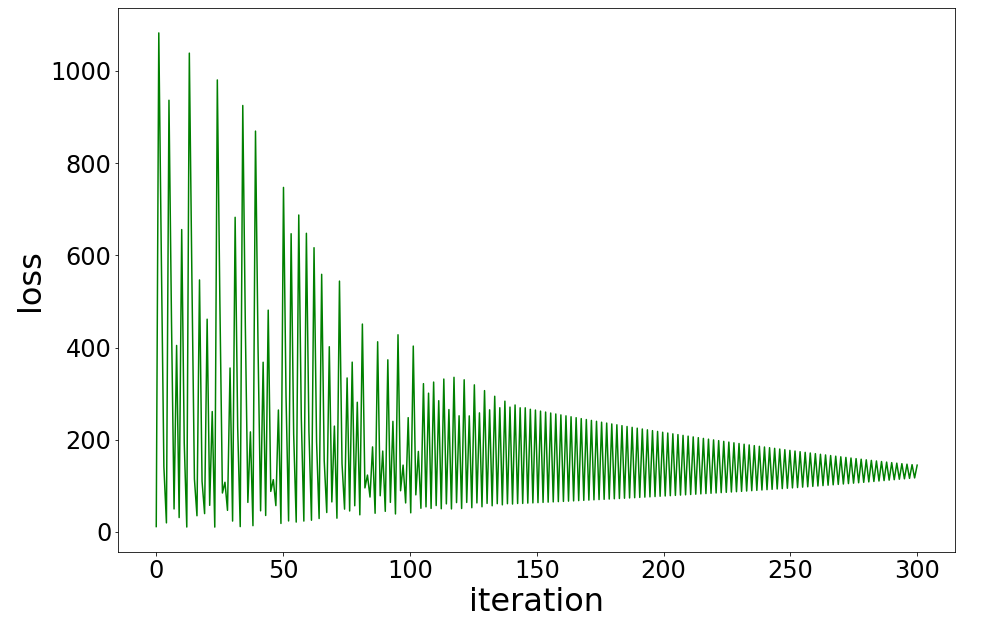
\includegraphics[width=\linewidth/2]{gd_loss.png}
		\caption{GD算法 损失率-迭代次数图(学习率=0.5)}
	\end{figure}
	可以看到损失率在波动范围内不断下降. 但显然这个波动太大了, 这是由于\textbf{学习率过高引起的}, 因此降低学习率到0.1, 得到以下图:
	\begin{figure}[H]
		\centering
		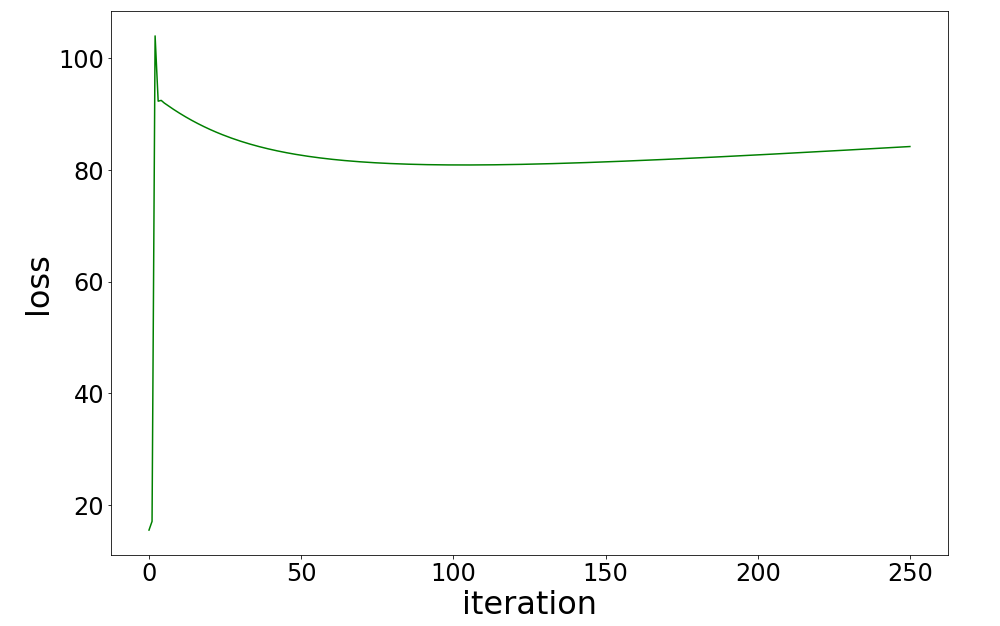
\includegraphics[width=\linewidth/2]{gd_loss_01.png}
		\caption{GD算法 损失率-迭代次数图(学习率=0.1)}
	\end{figure}
	\item 经过调整参数, 可以得到在\textbf{学习率为 0.1, epoch为300时}, 能够在\textbf{训练集上达到0.94的准确率}, 在\textbf{测试集上达到 1.0 的准确率}.
	\item 训练结果可视化. 从图中可以看出来, 测试集上的绿色线将两类样本都划分开来了.
	\begin{figure}[H]
		\begin{minipage}[H]{0.5\linewidth}
			\centering
			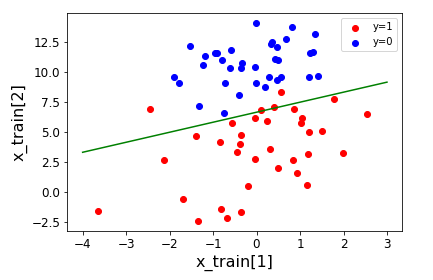
\includegraphics[width=\linewidth]{gd_train.png}
			\caption{GD算法在训练集上的表现}
		\end{minipage}
		\begin{minipage}[H]{0.5\linewidth}
			\centering
			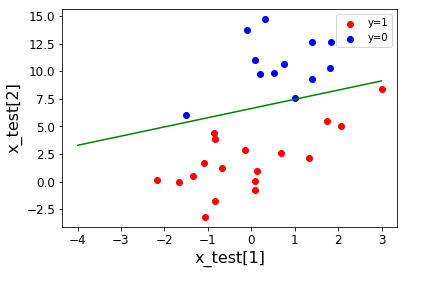
\includegraphics[width=\linewidth]{gd_test.png}
			\caption{GD算法在测试集上的表现}
		\end{minipage}
	\end{figure}
\end{itemize}
\subsection{SGD算法实验结果}
\begin{itemize}
	\item 经过调整参数, 可以得到在\textbf{学习率为 0.1, epoch为 5000 时}, 能够在\textbf{训练集上达到0.97的准确率}, 在\textbf{测试集上达到 0.93 的准确率}.
	\item 训练结果可视化:
	\begin{figure}[H]
		\begin{minipage}[H]{0.5\linewidth}
			\centering
			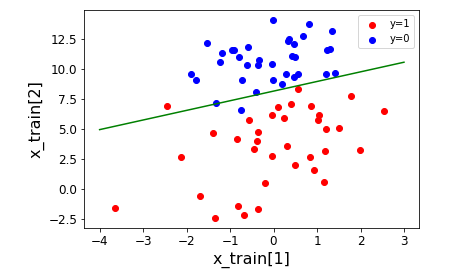
\includegraphics[width=\linewidth]{sgd_train.png}
			\caption{SGD算法在训练集上的表现}
		\end{minipage}
		\begin{minipage}[H]{0.5\linewidth}
			\centering
			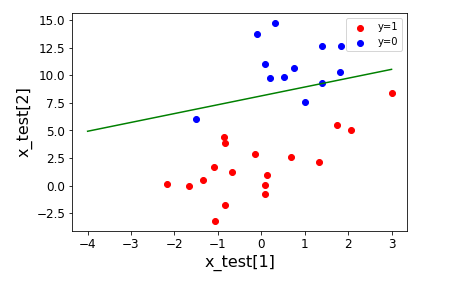
\includegraphics[width=\linewidth]{sgd_test.png}
			\caption{SGD算法在测试集上的表现}
		\end{minipage}
	\end{figure}
\end{itemize}
\subsection{Newton法实验结果}
\begin{itemize}
	\item 经过调整参数, 可以得到在\textbf{学习率为 0.1, epoch为200时}, 能够在\textbf{训练集上达到0.94的准确率}, 在\textbf{测试集上达到 1.0 的准确率}.
	\item 训练结果可视化. 从图中可以看出来, 测试集上的绿色线将两类样本都划分开来了.
	\begin{figure}[H]
		\begin{minipage}[H]{0.5\linewidth}
			\centering
			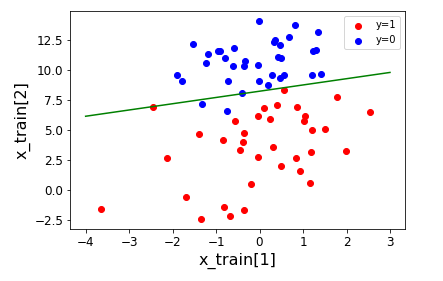
\includegraphics[width=\linewidth]{newton_train.png}
			\caption{Newton法在训练集上的表现}
		\end{minipage}
		\begin{minipage}[H]{0.5\linewidth}
			\centering
			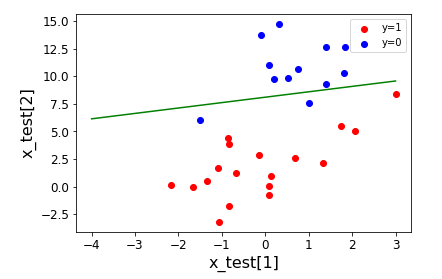
\includegraphics[width=\linewidth]{newton_test.png}
			\caption{Newton法在测试集上的表现}
		\end{minipage}
	\end{figure}
\end{itemize}
\subsection{sklearn 实验结果}
\noindent 直接调用sklearn能够得到在训练集上 0.957, 在测试集上 0.933 的效果
\begin{figure}[H]
	\begin{minipage}[H]{0.5\linewidth}
		\centering
		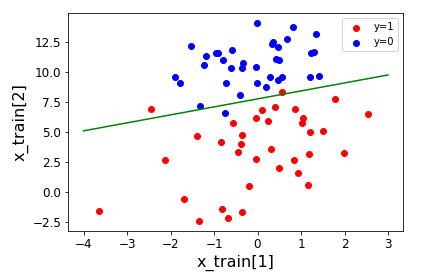
\includegraphics[width=\linewidth]{sklearn_train.png}
		\caption{调用sklearn在训练集上的表现}
	\end{minipage}
	\begin{minipage}[H]{0.5\linewidth}
		\centering
		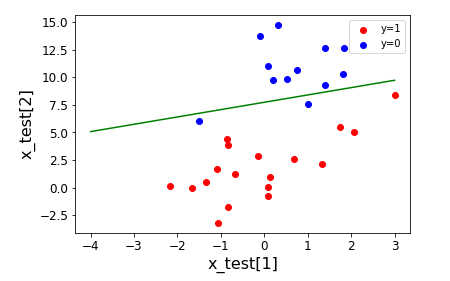
\includegraphics[width=\linewidth]{sklearn_test.png}
		\caption{调用sklearn在测试集上的表现}
	\end{minipage}
\end{figure}

\newpage
\section{附录: 实验代码}
\subsection{对率回归算法代码(包括GD,SGD,Newton)}
\begin{lstlisting}[language=python, caption=对率回归算法代码]
import numpy as np

x_train = np.load("./data/LR/train_data.npy")
y_train = np.load("./data/LR/train_target.npy")
x_test = np.load("./data/LR/test_data.npy")
y_test = np.load("./data/LR/test_target.npy")

class LogitRegression:
    def __init__(self, x_train, y_train, alpha=0.2, epoch=-1, tol=1e-2, model='GD'):
        self.x_train = x_train
        self.y_train = y_train
        self.beta = np.ones(x_train.shape[1])
        self.beta = np.random.uniform(low=0, high=1, size=x_train.shape[1])
        self.alpha = alpha
        self.epoch = epoch
        self.tol = tol
        self.model = model
        
    def probability(self, x):
        return 1/(1+np.exp(-x @ self.beta))
    
    def loss_J(self):
        p = self.probability(self.x_train)
        return -np.sum([self.y_train[i] * np.log(p[i]) + (1-self.y_train[i]) * np.log(p[i])
                        for i in range(len(self.y_train))])
    
    @property
    def m(self):
        return len(self.y_train)
    
    def train(self):
        # stop by tol
        loss = []
        if self.model == 'GD':
            if self.epoch == -1:
                while True:
                    grad = np.zeros(self.x_train.shape)
                    for i in range(self.m):
                        grad[i] = (1/(1+np.exp(-self.x_train[i] @ self.beta)) - self.y_train[i]) * self.x_train[i]
                    delta = self.alpha * grad.mean(axis=0)
                    self.beta -= delta
                    if np.abs(delta).mean() < self.tol:
                        break
                return

            # stop by epoch
            for _ in range(self.epoch):
                grad = np.zeros(self.x_train.shape)
                loss.append(self.loss_J())
                for i in range(self.m):
                    grad[i] = (1/(1+np.exp(-self.x_train[i] @ self.beta)) - self.y_train[i]) * self.x_train[i]
                self.beta -= self.alpha * grad.mean(axis=0)
            return loss
        elif self.model == 'SGD':
            # stop by epoch
            for _ in range(self.epoch):
                loss.append(self.loss_J())
                i = int(np.random.uniform(low=0, high=self.m-1, size=1))
                grad = (1/(1+np.exp(-self.x_train[i] @ self.beta)) - self.y_train[i]) * self.x_train[i]
                self.beta -= self.alpha * grad
            return loss
        elif self.model == 'newton':
            # stop by epoch
            for _ in range(self.epoch):
                grad = np.zeros(self.x_train.shape)
                gradd = np.zeros(1)
                loss.append(self.loss_J())
                for i in range(self.m):
                    expxbeta = np.exp(-self.x_train[i] @ self.beta)
                    grad[i] = (1/(1+expxbeta) - self.y_train[i]) * self.x_train[i]
                    gradd += (1/(1+expxbeta)) * (1-1/(1+expxbeta))
                self.beta -= self.alpha * grad.mean(axis=0) / gradd
            return loss
            
            
    def test(self, x_test, y_test):
        x_test = np.array(x_test)
        p = self.probability(x_test)
        acc = 1-np.sum(np.abs([float(round(i)) for i in lr.probability(x_test)] - y_test)) / len(y_test)
        return p, acc
    
    def get_xxyy(self, span):
        xx = np.linspace(*span, (span[1]-span[0])*100)
        yy = (-self.beta[0]-self.beta[1]*xx) / self.beta[2]
        return xx, yy

lr = LogitRegression(x_train, y_train, alpha=0.5, epoch=300, model='GD')
loss = lr.train()

print(lr.test(x_train, y_train)[1])
print(lr.test(x_test, y_test)[1])
\end{lstlisting}
\subsection{绘图代码}
\begin{lstlisting}[language=python, caption=绘图代码]
import matplotlib.pyplot as plt

xx, yy = lr.get_xxyy((-4, 3))
plt.xlabel('x_train[1]', size=16)
plt.ylabel('x_train[2]', size=16)
plt.xticks(size=12)
plt.yticks(size=12)
red = np.where(y_train == 1)
blue = np.where(y_train == 0)
plt.scatter(x_train[red][:, 1], x_train[red][:, 2], c='red', label='y=1')
plt.scatter(x_train[blue][:, 1], x_train[blue][:,2], c='blue', label='y=0')
plt.legend()
plt.plot(xx, yy, c='green')
\end{lstlisting}

\end{document}





